\documentclass[]{article}
\usepackage[MeX]{polski} 
\usepackage[utf8]{inputenc} 
\usepackage{lipsum}
\usepackage{graphicx}
\usepackage{wrapfig}


\title{dokument  \LaTeX}
\author{Imię Nazwisko}
\date{Styczeń 2024}

\begin{document}

\maketitle

\begin{abstract}
  To jest streszczenie tego dokumentu.
\end{abstract}

\tableofcontents

\newpage

\section{Matematyka}
\textbf{Matematyka } – nauka zaliczana do grupy formalnych, inaczej dedukcyjnych lub apriorycznych, a także do nauk ścisłych i definiująca tę grupę – matematyka stanowi ich fundament. Dotyczy ona ścisłych wniosków z przyjętych założeń – prawidłowości rozumowania, podobnie jak logika, jednak matematyka się z nią nie pokrywa. Ścisłe założenia mogą dotyczyć najróżniejszych dziedzin myśli ludzkiej; muszą być czynione w naukach ścisłych, technice i zdarzają się w naukach humanistycznych, przez co zakres matematyki stale się powiększa razem z tymi naukami. 
\begin{flushright}
\scriptsize
Żródło: https://pl.wikipedia.org/wiki/Matematyka
\end{flushright}


\subsection{Równania matematyczne}
    \begin{table}[h!]
    \centering
	\begin{tabular}{|c|c|}
	\hline
	Nazwa & Równanie \\
	\hline
	Równanie Maxwella & $\nabla \times \vec{E} = - \frac{\partial \vec{B}}{\partial t}$ \\
	\hline
	Równanie Schrödingera & $i\hbar\frac{\partial}{\partial t}\psi(\vec{r},t) = \hat{H}\psi(\vec{r},t)$ \\
	\hline
	Równanie Laplace'a & $\nabla^2 f(\vec{r}) = 0$ \\
	\hline
	Równanie różniczkowe ruchu Browna & $\frac{\partial}{\partial t}P(\vec{r},t) = D\nabla^2 P(\vec{r},t)$ \\
	\hline
	Równanie Falowe & $\frac{\partial^2 u(x,t)}{\partial x^2} = \frac{1}{v^2}\frac{\partial^2 u(x,t)}{\partial t^2}$ \\
	\hline
\end{tabular}
  \label{tab:tabela}
\end{table}
\newpage
\subsection{Liczba PI}
\textbf{PI} - stosunek obwodu koła (czyli długości okręgu) do długości jego średnicy; stosunek ten jest niezależny od wielkości koła, bowiem wszystkie koła są do siebie podobne. 
\begin{flushright}
\scriptsize
Żródło: https://pl.wikipedia.org/wiki/Pi
\end{flushright}

    \begin{figure}[h]
    \centering
    
\includegraphics[width=0.5\textwidth]{pi.png}
    \caption{liczba pi}
    \label{img:liczbapi}
    \end{figure}

\newpage 

\section{Lorem Ipsum}
	\begin{wrapfigure}{r}{0.5\textwidth}
  \centering
  \includegraphics[width=0.48\textwidth]{left.png}
  \caption{Airbus a320neo}
  \label{img:a320nairportl}
\end{wrapfigure}
    \subsection{\underline{Lorem Ipsum}}
    \lipsum[1-7]
	\begin{figure}{h}
  \centering
  \includegraphics[width=0.48\textwidth]{right.png}
  \caption{Airbus a320neo}
  \label{img:a320nairportr}
\end{figure}
\newpage
    \subsection{\underline{Dolor Sit Amet}}
    \lipsum[7-14]

\newpage
    \subsection{\underline{Consecteuer Adipiscing Elit!}}
    \lipsum[15-19]
   
\begin{wrapfigure}{r}{0.5\textwidth}
  \centering
  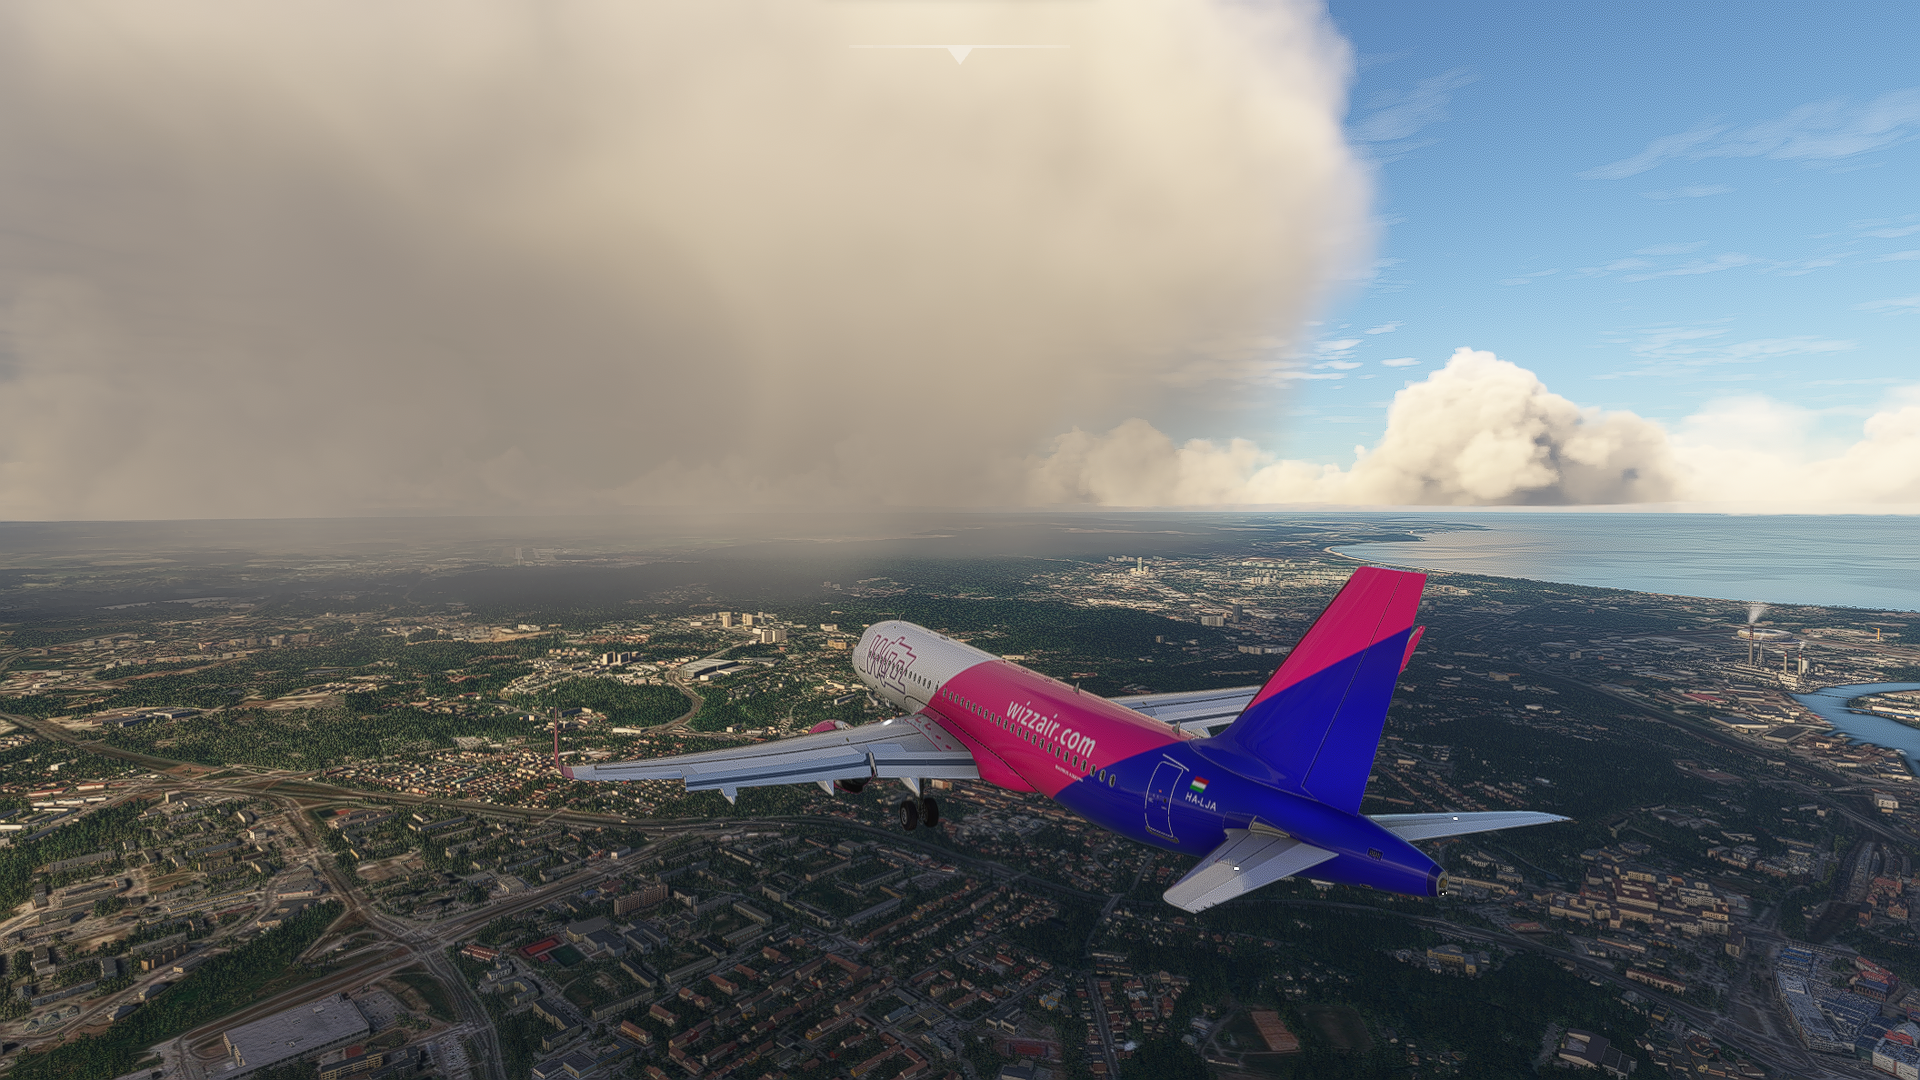
\includegraphics[width=0.48\textwidth]{landing.png}
  \caption{Airbus a320neo}
  \label{img:a320n}
\end{wrapfigure}

\newpage
    \subsection{\underline{Nulla Ac Nisl}}
    \lipsum[20-22] \\

\section{Podsumowanie}
Użyłem Rysunku \ref{img:liczbapi}, Rysunku \ref{img:a320nairportl}, Rysunku \ref{img:a320nairportr}, Rysunku \ref{img:a320n} i Tabeli \ref{tab:tabela}.

\section{Bibliografia}
1.  https://pl.wikipedia.org/wiki/Matematyka
\newline
2.  https://pl.wikipedia.org/wiki/Pi


\end{document}